\chapter{Introducción}\label{Int}
%Función que crea el título de capítulo y al cual se le da el nombre deseado a través de su parámetro obligatorio. Al no tener la función el “*” se escribirá también en el título del documento las palabras “Capítulo 1: …”. Además se indica, mediante la función “\label”, la correspondiente etiqueta que lleva asociada. La etiqueta sirve para que en caso de que luego se quiera hacer referencia al capítulo se haga llamando etiqueta tal que se escribiría “La información correspondiente a dicho tema se encuentra en el capítulo \ref{Int}.”

\thispagestyle{fancy}
%Función que determina que durante este capítulo se aplique el estilo Fancy.

\fancyhead[LE]{\thechapter.NOMBRE DEL PRIMER CAPÍTULO} 
%Función que se utiliza para indicar que en las páginas impares, aparezca en el encabezado en la parte izquierda, el número del capítulo con su correspondiente nombre.

Lorem ipsum dolor sit amet, consectetur adipiscing elit. Fusce bibendum mauris metus, quis pellentesque nisl vestibulum ut. Cras finibus, tortor id mattis imperdiet, tellus risus consectetur nisi, et luctus neque nisl nec massa. Sed interdum lacus eget nisl porttitor mattis. Donec volutpat blandit tortor ut porttitor. Integer nec pulvinar sapien. Integer eget odio feugiat, pretium tortor vel, dictum est. Proin ac eleifend augue, vitae facilisis dolor. Suspendisse at augue maximus, maximus est in, posuere dui. Nam id lorem et leo vehicula faucibus. Proin ac nunc sit amet metus ullamcorper fringilla non in quam. Sed at condimentum enim.\\
%Texto sin sentido y predeterminado que se irá utilizando a lo largo de todo el documento para simular la escritura de la memoria.

\setlength{\fboxsep}{5pt}
\begin{figure}[thbp]
\centering
\fbox{
\includegraphics[width=0.6\textwidth, height=3.8cm]{Figuras/LDeusto.jpeg}}
\caption{Logo de Deusto (Fuente: Universidad de Deusto \cite{Deusto}} \label{fig:Deusto}
\end{figure}
%Todas estas funciones aparecen explicadas con detalle en el documento "Funciones.tex".

\textcolor{Rojo}{Como se puede observar en la imagen \ref{fig:Deusto}}: Cras neque purus, vulputate at neque a, rutrum elementum odio. Sed ultrices enim nulla, ac consectetur enim malesuada maximus. Nulla facilisi. Curabitur pharetra tortor nisl, vel molestie turpis commodo eget. Morbi viverra urna varius, condimentum nulla eu, semper mi. Aenean faucibus erat id felis consequat, sit amet porttitor nibh posuere. Proin imperdiet fermentum odio eget aliquet. Aenean quis auctor ante, ut consequat nunc. Maecenas ac lacinia risus. Donec finibus erat in mattis pharetra. Morbi sed metus eget magna luctus placerat quis eget velit. Praesent imperdiet velit ut magna bibendum pretium. Vestibulum fermentum nulla et suscipit tempor. Vestibulum facilisis vulputate faucibus. Vivamus et elementum tellus, at accumsan augue. Fusce elementum sem ut nunc efficitur ullamcorper. Sed ac erat quis massa pellentesque gravida id sit amet nulla. Nunc ultricies porttitor metus at fermentum \cite{Deusto}.\\

\setlength{\fboxsep}{0pt}
%"\Fbox" es una función que como se verá posteriormente es utilizada para recuadrar fotos o enmarcarlas con un borde negro. Esta función indica que no haya separación entre la foto y el marco, es decir, que justo aparezca el marco cuando acabe la foto. Se puede cambiar el "0pt" por otro número y se dejará un espacio alrededor de la foto hasta que comience el marco.

\begin{figure}[H]
\centering
\begin{minipage}[h]{.48\linewidth}
\vspace{1.5cm}
\centering
\fbox{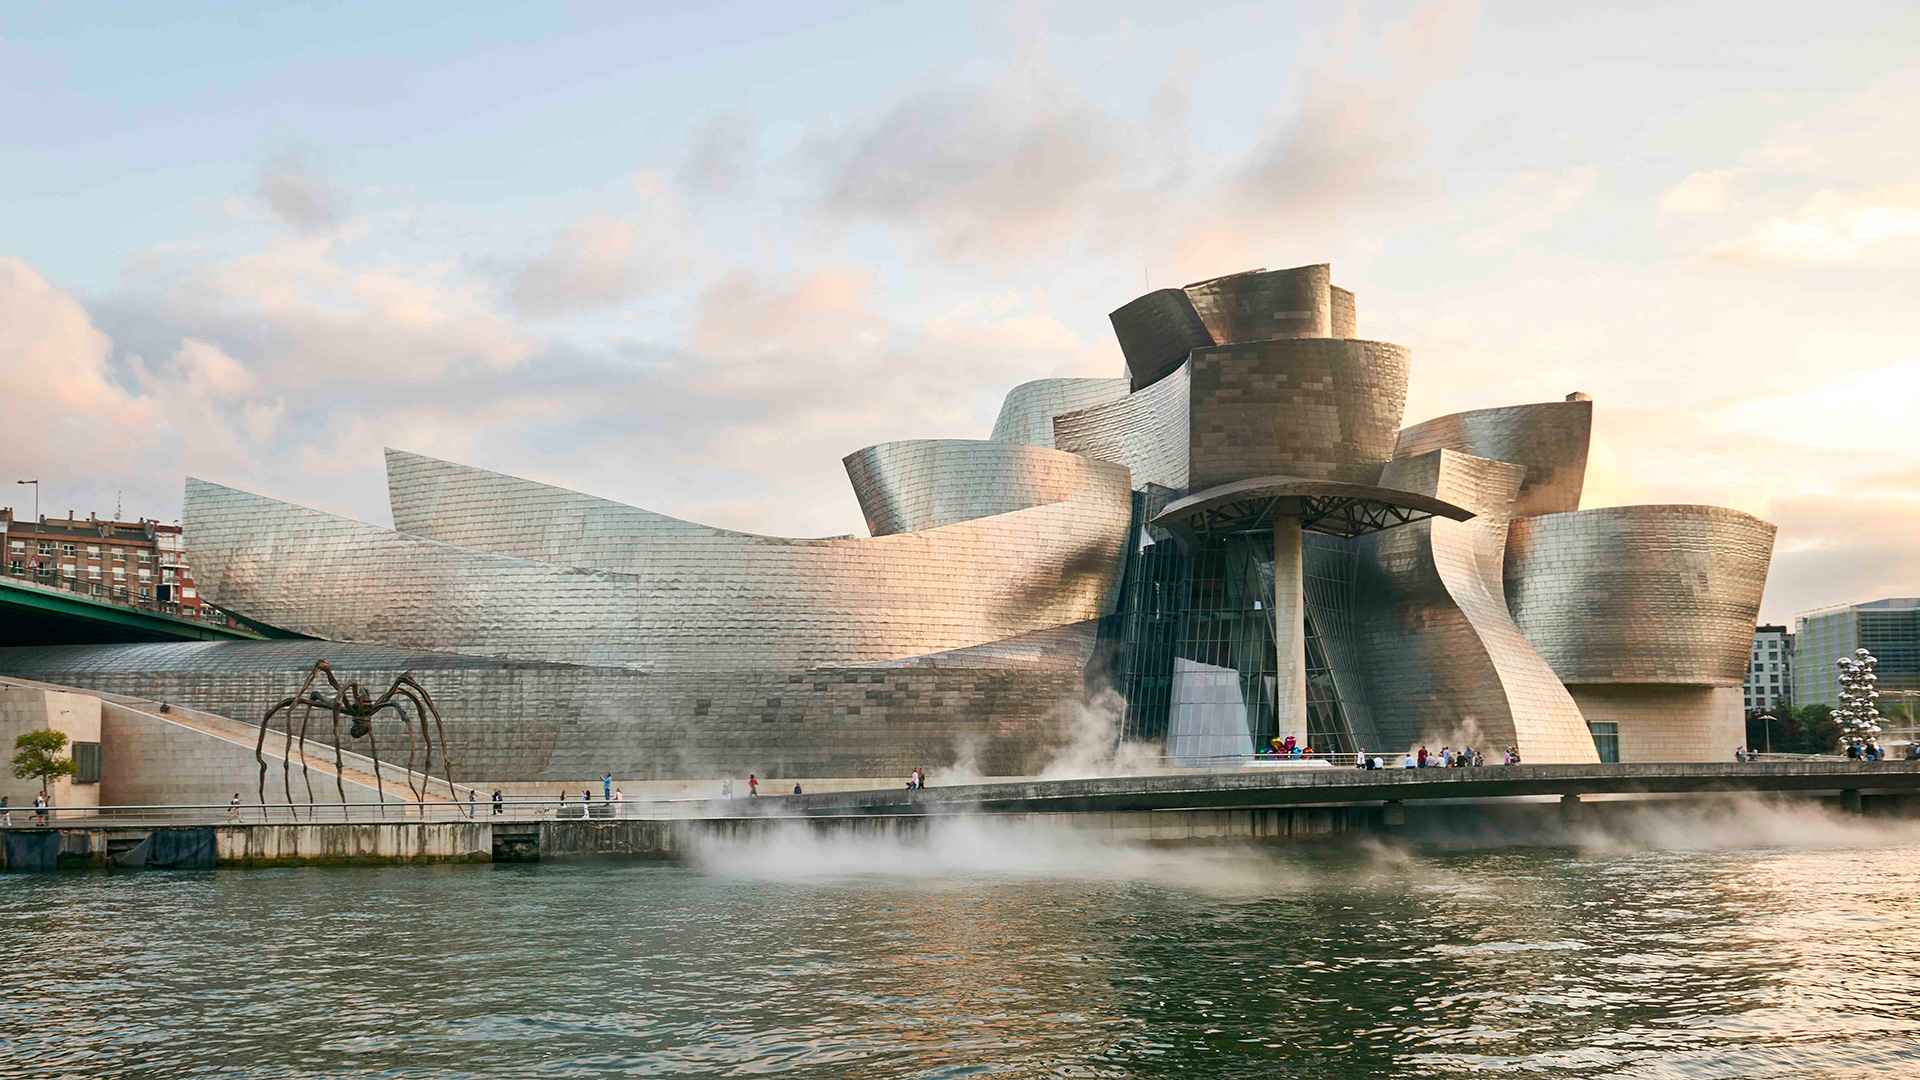
\includegraphics[width=\textwidth, height=4.5cm]{Figuras/Gugg.jpg}}
\caption{Guggenheim - Bilbao (Fuente: Google \cite{Gugg}).} \label{fig:Gugg}
\end{minipage}
\hfill
\begin{minipage}[h]{.45\linewidth}
\centering
\fbox{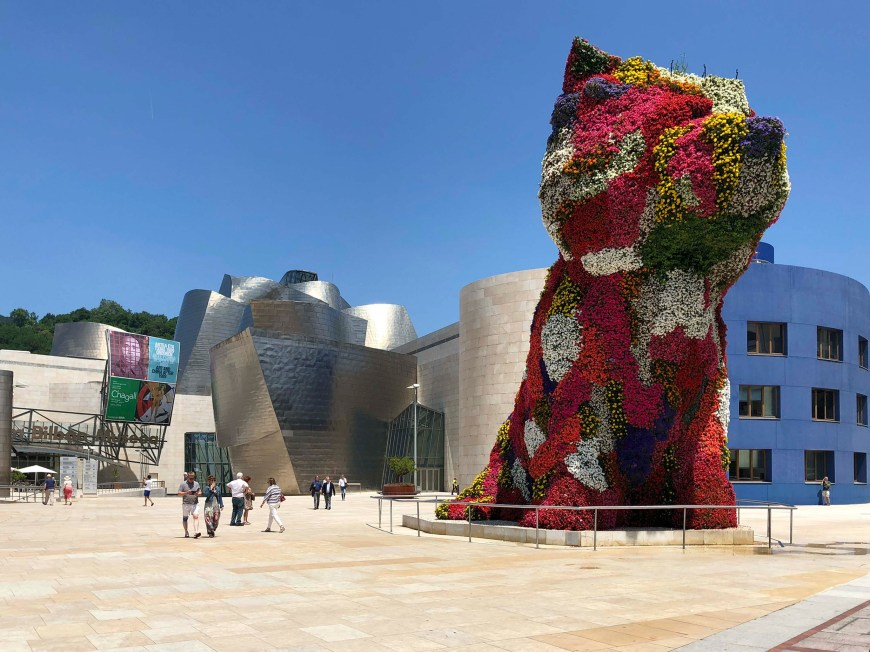
\includegraphics[width=\textwidth, height=6cm]{Figuras/Puppy.jpg}}
\caption{Puppy - Guggenheim (Fuente: Google \cite{Puppy}).} \label{fig:Puppy}
\end{minipage}
\end{figure}

Cras efficitur purus ut ante sollicitudin, vel vulputate enim pulvinar. Suspendisse sit amet erat ut dui accumsan pharetra eget in arcu. Vestibulum fermentum a velit ac cursus. In tempus elit risus, a vestibulum est viverra a. Vestibulum ut nulla venenatis, congue urna quis, ullamcorper lacus. Duis ac hendrerit nisi, id imperdiet purus. Proin non iaculis sem. Suspendisse potenti. Nulla sed dui orci. Pellentesque vel feugiat quam, non eleifend purus. Donec porttitor velit vel sollicitudin cursus. Vivamus rhoncus vel risus non vestibulum. Aenean fermentum congue pretium. Donec dolor felis, iaculis iaculis gravida vitae, placerat ac enim.

\section{Sección}
Etiam interdum lectus nec elementum consequat. Maecenas at enim et ante aliquet porta pellentesque vitae libero. Integer tortor magna, efficitur in mauris vel, cursus consectetur magna. Donec nec nibh ultricies, ultricies velit interdum, porta nibh. Curabitur ornare, ex nec finibus interdum, leo felis semper dui, vitae auctor velit libero at arcu. In hendrerit tortor quis tempus efficitur. Aenean vel feugiat nisi, quis sagittis ex. Duis sit amet blandit ligula. Curabitur quis enim nibh. Nulla facilisi. Nunc nec dictum libero. Sed mattis euismod nulla et bibendum.

\begin{itemize}
\renewcommand{\labelitemi}{$\bullet$}
\setlength{\itemindent}{5mm}
    \item Curabitur ullamcorper varius congue.
    \item Vivamus eu quam sem. Aenean a ligula a est blandit dignissim vel non odio.
    \item Etiam sit amet velit quis enim porta semper sit amet vitae diam.
\end{itemize}

\subsection{Subsección}
In bibendum urna libero, ut maximus ex pharetra non. Aliquam sed metus eget lacus suscipit bibendum eget sed risus. Aenean dictum, urna eu lobortis auctor, quam sem porta ex, ut dignissim lectus sapien et dui. Phasellus eros massa, imperdiet vitae elit et, malesuada feugiat odio. Vivamus interdum turpis sit amet ligula rhoncus semper. Curabitur nec consequat libero, at suscipit neque. Donec commodo arcu vel eros feugiat, vitae hendrerit risus efficitur. Nulla convallis ex sed nisi ullamcorper feugiat.\\

\renewcommand{\arraystretch}{1.6}
\begin{table}[]
\begin{center}
\begin{tabular}{|m{7cm}| m{7cm} |}
\hline
\rowcolor{Cyan}
\centering \textbf{Lorem ipsum} & \hspace{2.75cm} \textbf{Dolor sit} \\\hline
\textbf{Consectetur adipiscing} & Elit\\ \hline
\rowcolor{GrisTabla}
\textbf{Consectetur adipiscing} & Elit \\ \hline
\textbf{Consectetur adipiscing} & Elit \\ \hline
\rowcolor{GrisTabla} 
\textbf{Consectetur adipiscing} & Elit \\ \hline
\rowcolor{Naranja} 
\textbf{In bibendum urna} & \textbf{Libero} \\ \hline
\end{tabular}
\caption{Tabla con texto por defecto (Fuente: Elaboración propia).}
\label{Medioambiente}
\end{center}
\end{table}

\subsubsection{Subsubsección}

Lorem ipsum dolor sit amet, consectetur adipiscing elit. Phasellus scelerisque sem quis sem commodo dictum. Maecenas venenatis hendrerit tortor, eget maximus dui ultrices ac. Vivamus aliquam ipsum non tellus lacinia varius. Nunc dapibus porta commodo. Praesent et porttitor nibh. Nunc consectetur congue dolor, ut venenatis leo. Suspendisse potenti. Nunc non nisi a metus vestibulum euismod. Vivamus dapibus lobortis sagittis. Fusce tincidunt neque velit, sed gravida ex interdum vel.\\

Ut commodo suscipit aliquet. Phasellus accumsan rhoncus lectus sit amet blandit. Duis nec quam et sapien blandit volutpat. Pellentesque nec nisl non tellus aliquet facilisis. Quisque dictum arcu quis leo blandit pulvinar non non nisi. Vivamus accumsan nec enim at scelerisque. Vestibulum ante ipsum primis in faucibus orci luctus et ultrices posuere cubilia Curae; Suspendisse hendrerit tellus ut massa sagittis, in pellentesque odio pulvinar. Sed tristique viverra mi, vitae ornare orci vestibulum eu. Nunc quis elit ante.\\
\newpage
\thispagestyle{empty}